\subsection{Absorption von $\gamma$-Strahlung}
Für den theoretischen Wert des Absorptionskoeffizient wird zunächst der Compton'sche Wirkungsquerschnitt nach Gleichung \eqref{eqn:sigma} berechnet.
Dafür ist das Verhältnis von Quantenenergie des $^{137}Cs$ zur Ruheenergie des Elektrons gegeben \cite{1}:
\begin{align*}
  \epsilon=\SI{1.295}{}.
\end{align*}
Damit ergibt sich der Compton'sche Wirkungsquerschnitt zu:
\begin{align*}
  \sigma_{\text{com}}= \SI{2.566e-29}{\frac{1}{m}}.
\end{align*}
Die beiden verwendeten Absorber sind Eisen und Blei mit den folgenden Eigenschaften \cite{fe}, \cite{pb}:
\begin{table}[h!]
  \centering
  \caption{Parameter zu den Materialien Blei und Eisen}
  \label{tab:par}
  \begin{tabular}{c c c}
    \toprule
    & Eisen & Blei  \\
    \midrule
    Z      & 26                   & 82 \\
    M      & $\SI{55,845}{u N_{A}}$       & $\SI{207,2}{u N_{A}}$ \\
    $\rho$ & $\SI{7874}{\frac{kg}{m^3}}$  & $\SI{11342}{\frac{kg}{m^3}}$ \\

    \bottomrule
  \end{tabular}
\end{table}

Dabei ist $u=\SI{1.6605e-27}{kg}$ die Atomare Masseneinheit und $N_{\text{A}}=\SI{6.022e23}{\frac{1}{mol}}$ \cite{taschenrechner}.
Die Absorptionskoeffizienten berechnen sich nach Gleichung \eqref{eqn:koeff} zu:
\begin{align*}
  \mu_{\text{com, Fe}}= \SI{56.647}{\frac{1}{m}}\\
  \mu_{\text{com, Pb}}= \SI{69.360}{\frac{1}{m}}.\\
\end{align*}
Ein statistischer Fehler der Zählrate in der Strahlenphysik berechnet sich über
\begin{align*}
  \Delta N = \sqrt{N}
\end{align*}
\\Die Hintergrundstrahlung wird als
\begin{align*}
   N_{\text{U1}}=\SI{1229\pm35}{}
\end{align*}
Impulse innerhalb $t_{\text{U1}}=\SI{1000}{s}$ gemessen. Damit ergibt sich die Rate
\begin{align*}
  \frac{N_{\text{U1}}}{t_{\text{U1}}}=\SI{1.229 \pm 0.035}{\frac{1}{s}}
\end{align*}
Die Messwerte zur Absorption der $\gamma$-Strahlung sind für den Absorber Blei und den Absorber Eisen in den Tabellen \ref{tab:pb} und \ref{tab:fe} notiert.
In den Abbildungen \ref{fig:pb} und \ref{fig:fe} sind die Messwerte absorberabhängig aufgetragen.
\begin{figure}[h!]
  \centering
  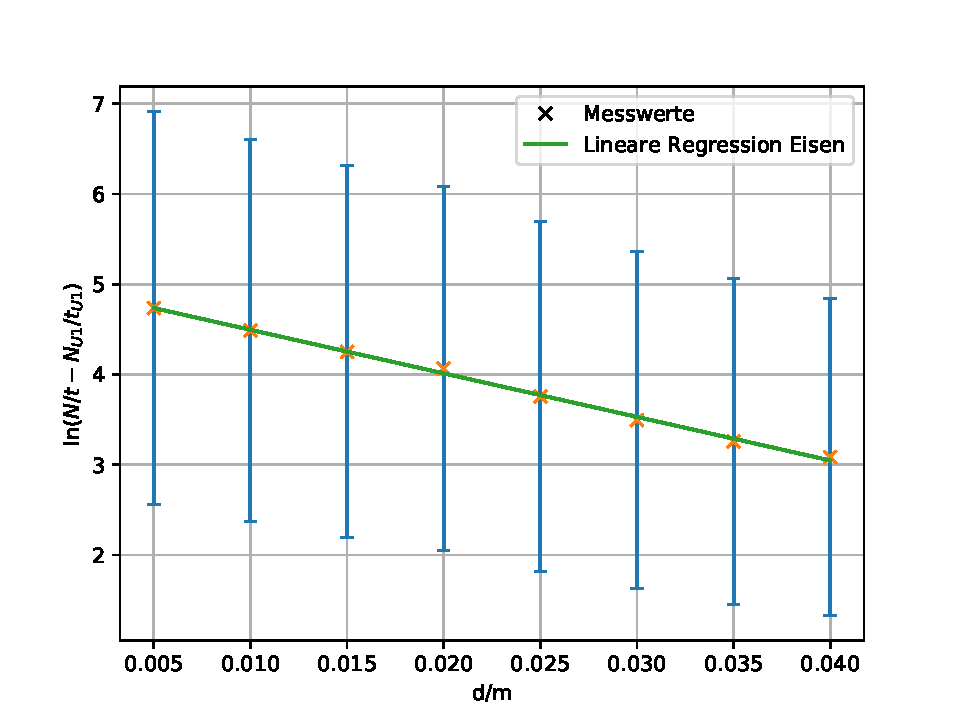
\includegraphics[width=\textwidth]{fe.pdf}
  \caption{Absorptionskurve $\beta$-Strahlung für Eisen}
  \label{fig:fe}
\end{figure}
\begin{figure}[h!]
  \centering
  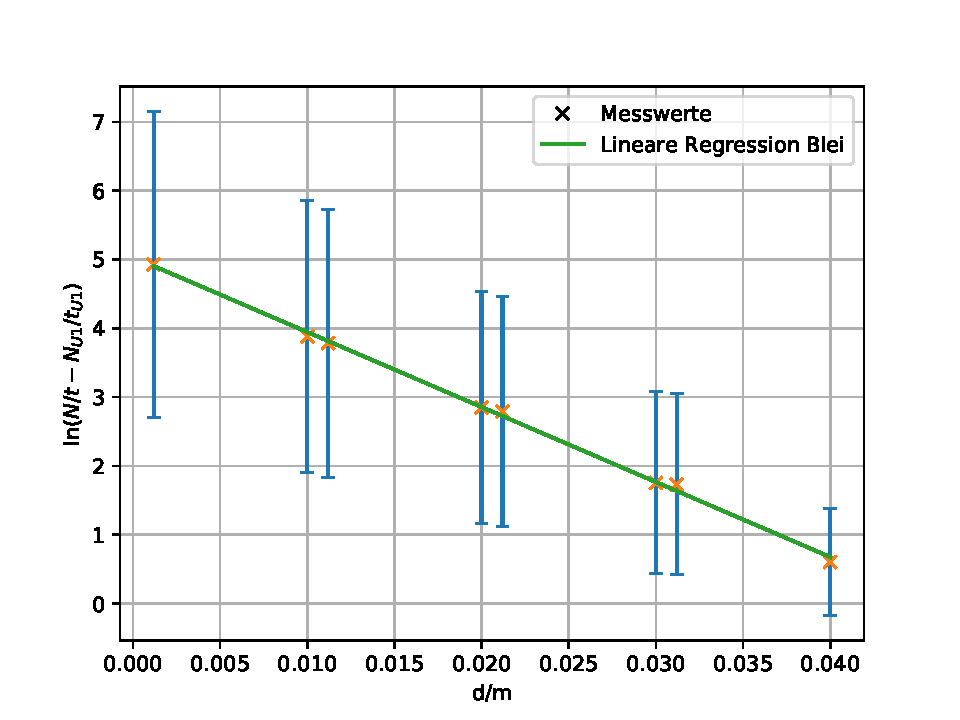
\includegraphics[width=\textwidth]{pb.pdf}
  \caption{Absorptionskurve $\beta$-Strahlung für Blei}
  \label{fig:pb}
\end{figure}
\begin{table}[h!]
  \centering
  \caption{Messdaten zur Absorption der $\gamma$-Strahlung in Eisenplatten}
  \label{tab:fe}
  \begin{tabular}{c c c c c c}
    \toprule
    d/m &  $N$  & $t/s$ & $\frac{N}{t}/\frac{1}{s}$ & $\frac{N}{t}-\frac{N_{\text{U1}}}{t_{\text{U1}}}/ \frac{1}{s}$ &  $\ln{\left( \frac{N}{t}-\frac{N_{\text{U1}}}{t_{\text{U1}}} \right)} $ \\
    \midrule
    0,005 & 5760 & 50  & 115,2  &  113,974 &  4,736 \\
    0,01  & 5396 & 60  & 89,933 &  88,707  &  4,485 \\
    0,02  & 4460 & 75  & 59,467 &  58,241  &  4,065 \\
    0,015 & 6712 & 94  & 71,404 &  70,178  &  4,251 \\
    0,025 & 5512 & 125 & 44,096 &  42,87   &  3,758 \\
    0,03  & 4605 & 135 & 34,111 &  32,885  &  3,493 \\
    0,035 & 3956 & 145 & 27,283 &  26,057  &  3,260 \\
    0,04  & 3578 & 155 & 23,084 &  21,858  &  3,085 \\

    \bottomrule
  \end{tabular}
\end{table}

\begin{table}[h!]
  \centering
  \caption{Messdaten zur Absorption der $\gamma$-Strahlung in Bleiplatten}
  \label{tab:pb}
  \begin{tabular}{c c c c c c}
    \toprule
    d/m  & $N$  & $t/s$ & $\frac{N}{t}/\frac{1}{s}$ & $\frac{N}{t}-\frac{N_{\text{U1}}}{t_{\text{U1}}}/ \frac{1}{s}$ & $\ln{\left( \frac{N}{t}-\frac{N_{\text{U1}}}{t_{\text{U1}}} \right)} $  \\
    \midrule
    0,0012 & 6975   &   50    &  139,5  & 138,274 & 4,929 \\
    0,01   & 4976   &  100    &  49,76  & 48,534  & 3,882 \\
    0,02   & 3693   &  200    &  18,465 & 17,239  & 2,847 \\
    0,0112 & 6776   &  150    &  45,173 & 43,947  & 3,783 \\
    0,0212 & 4402   &  250    &  17,608 & 16,382  & 2,796 \\
    0,03   & 2107   &  300    &  7,023  & 5,797   & 1,757 \\
    0,0312 & 2410   &  350    &  6,886  & 5,660   & 1,733 \\
    0,04   & 1220   &  400    &  3,05   & 1,824   & 0,601 \\

    \bottomrule
  \end{tabular}
\end{table}

Die lineare Regressionen der Form $y=ax+b$ der Messwerte mittels Python liefern die Parameter
\begin{align*}
  &\text{Eisen}   &   \\
  &c= -\mu_{\text{Fe}} = &\SI{-48.245 \pm 1.054}{\frac{1}{m}}\\
  &d= &\SI{4.977 \pm 6.72e-04}{}\\
  &\text{Blei}    &   \\
  &a= -\mu_{\text{Pb}} = &\SI{-108.944 \pm 3.761}{\frac{1}{m}}\\
  &b= &\SI{5.035 \pm 2.14e-03}{}\\.
\end{align*}
Dabei entsprechen die Steigungen den negativen Absorptionskoeffizienten $-\mu$.
\FloatBarrier

\subsection{Absorption von $\beta$-Strahlung}
Als Dichte des Aluminiums wird
\begin{align*}
  \rho_{\text{Al}}=\SI{2.71}{\frac{g}{cm^3}}= \SI{2710}{\frac{kg}{m^3}}
\end{align*}
verwendet \cite{2}.
Die Massenbelegung $R$ berechnet sich mit Gleichung \eqref{eqn:massenbelegung}.
Die Messung der Hintergrundstrahlung ergibt sich zu
\begin{align*}
  N_{\text{U2}}= \SI{614 \pm 25}{}
\end{align*}
in $t_{\text{U2}}=\SI{1000}{s}$.
Damit errechnet sich die Zählrate zu
\begin{align*}
  \frac{N_{\text{U2}}}{t_{\text{U2}}}=\SI{0.614 \pm 0.025}{\frac{1}{s}}
\end{align*}
Die Messwerte zur Absorption der $\beta$-Strahlung sind in Tabelle \ref{tab:beta} zu finden.
\begin{table}[h!]
  \centering
  \caption{Messdaten zur Absorption der $\beta$-Strahlung}
  \label{tab:beta}
  \begin{tabular}{c c c c c c c}
    \toprule
      d/ \SI{e-6}{m} & R/$\frac{kg}{m^2}$ & $N$  & $t/s$ & $\frac{N}{t}/\frac{1}{s}$ & $\frac{N}{t}-\frac{N_{\text{U2}}}{t_{\text{U2}}}/ \frac{1}{s}$ & $\ln{\frac{N}{t}-\frac{N_{\text{U2}}}{t_{\text{U2}}}}$  \\
    \midrule
    100          & 0,271                    & 2412  &   60    &   40,2    & 39,586 &  3,678   \\
    125          & 0,339                    & 608   &   60    &   10,133  & 9,519  &  2,253   \\
    153\pm0.5    & 0,415\pm \SI{1,355e-3}{} & 543   &   60    &   9,05    & 8,436  &  2,132   \\
    160\pm1      & 0,434\pm \SI{2,71e-3}{}  & 422   &   80    &   5,275   & 4,661  &  1,539   \\
    200\pm1      & 0,542\pm \SI{2,71e-3}{}  & 317   &   150   &   2,113   & 1,499  &  0,408   \\
    253\pm1      & 0,686\pm \SI{2,71e-3}{}  & 287   &   350   &   0,82    & 0,206  &  -1,580   \\
    302\pm1      & 0,818\pm \SI{2,71e-3}{}  & 442   &   600   &   0,737   & 0,123  &  -2,096   \\
    338\pm5      & 0,916\pm 0,014           & 411   &   600   &   0,685   & 0,071  &  -2,645   \\
    400\pm1      & 1,084\pm \SI{2,71e-3}{}  & 416   &   600   &   0,693   & 0,079  &  -2,538   \\
    444\pm2      & 1,203\pm \SI{5,42e-3}{}  & 424   &   600   &   0,707   & 0,093  &  -2,375   \\
    482\pm1      & 1,306\pm \SI{2,71e-3}{}  & 489   &   700   &   0,699   & 0,085  &  -2,465   \\


    \bottomrule
  \end{tabular}
\end{table}

Die Messwerte $R$ und die Intensität $\frac{N}{t}-\frac{N_{U}}{t_{U}}$ sind halblogarithmisch in Abbildung \ref{fig:beta} aufgetragen.
\begin{figure}[h!]
  \centering
  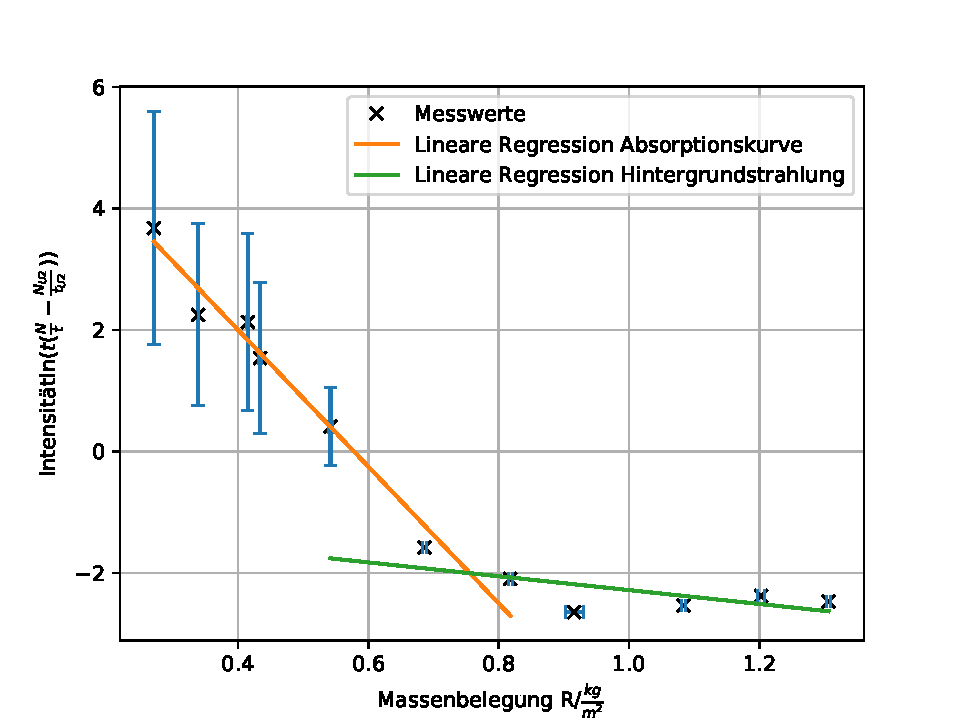
\includegraphics[width=\textwidth]{beta.pdf}
  \caption{Absorptionskurve $\beta$-Strahlung}
  \label{fig:beta}
\end{figure}
Die lineare Regression der Absorptionskurve der Form $y=ex+f$ (orange) mit Python liefert die Parameter
\begin{align*}
  e=& \SI{-11.255 \pm 2.670}{m^2/kg} \\
  f=& \SI{6.506 \pm 0.450}{}.
\end{align*}
Die lineare Regression der Hintergrundstrahlung der Form $y=gx+h$ (grün) mittels Python ergibt die Parameter
\begin{align*}
  g=& \SI{-1.141 \pm 0.358}{m^2/kg}\\
  h=& \SI{-1.140 \pm 0.376}{}.
\end{align*}
Der Schnittpunkt der beiden Geraden berechnet sich über $ex+f=gx+h$:
\begin{align*}
  R_{\text{max}}=x=\frac{h-f}{e-g}.
\end{align*}
Der Fehler berechnet sich über die Gauß'sche Fehlerfortpflanzung
\begin{align*}
  \Delta R_{\text{max}}&  =\sqrt{ \left( \frac{\partial x}{\partial e} \right)^2 \Delta e^2 + \left( \frac{\partial x}{\partial f} \right)^2 \Delta f^2 + \left( \frac{\partial x}{\partial g} \right)^2 \Delta g^2 + \left( \frac{\partial x}{\partial h} \right)^2 \Delta h^2 }\\
          &=\sqrt{ \left( \frac{f-h}{(e-g)^2} \right)^2\Delta e^2 + \left( -\frac{1}{e-g} \right)^2\Delta f^2 +\left( \frac{h-f}{(e-g)^2} \right)^2\Delta g^2 +\left( \frac{1}{e-g} \right)^2\Delta h^2} \\
          &= \SI{0.209}{kg/m^2}.
\end{align*}
Damit ergibt sich $R_{\text{max}}$ zu
\begin{align*}
  R_{\text{max}}=\SI{0.757 \pm 0.209}{kg/m^2}= \SI{0.0757 \pm 0.0209}{g/cm^2}.
\end{align*}
Als maximale Energie ergibt sich nach
\begin{align*}
  E_{\text{max}}= 1,92 \sqrt{R_{\text{max}}^2 + 0,22 R_{\text{max}}}= \SI{0.287}{MeV}
\end{align*}
Die Gauß'sche Fehlerfortpflanzung ergibt
\begin{align*}
  \Delta E_{\text{max}}=\sqrt{ \left( 1,92 \frac{0,22+2 R_{\text{max}}}{2 \sqrt{R_{\text{max}}(0,22 + R_{\text{max}})}} \right)^2 \Delta R_{\text{max}}^2}= \SI{0.050}{MeV}.
\end{align*}
Damit beläuft sich die maximale Energie zu
\begin{align*}
  E_{\text{max}}= \SI{0.287 \pm 0.050}{MeV}.
\end{align*}

\FloatBarrier
